%\documentclass[11pt,a4paper]{article}
\documentclass[11pt,a4paper]{book}
\usepackage[english]{babel}
\usepackage{graphicx,latexsym,isabelle,isabellesym,amssymb,pdfsetup}

% proper setup for best-style documents
\urlstyle{rm}
\isabellestyle{it}

\pagestyle{myheadings}

%make a bit more space
\addtolength{\hoffset}{-1,5cm}
\addtolength{\textwidth}{3cm}
\addtolength{\voffset}{-1cm}
\addtolength{\textheight}{2cm}

\renewcommand{\setisabellecontext}[1]{\markright{Theory~#1}}

\newcommand{\secref}[1]{Section~\ref{#1}}
\newcommand{\secrefs}[1]{Sections~\ref{#1}}
\newcommand{\charef}[1]{Chapter~\ref{#1}}
\newcommand{\charefs}[1]{Chapters~\ref{#1}}

%remove clutter from the toc
\setcounter{secnumdepth}{2}
\setcounter{tocdepth}{1}

\begin{document}

\title{JinjaDCI: a Java semantics with dynamic class initialization}
\author{Susannah Mansky}
\maketitle

%\begin{abstract}
%((FIXME: add abstract))
%\end{abstract}
\begin{trivlist}
\item \textbf{Abstract.}
This work is an extension of the Jinja semantics for Java and the JVM by Klein and Nipkow to include static fields and methods and dynamic class initialization.
In Java, class initialization methods are run dynamically, called when classes are first used. Such calls are handled by the running of an initialization procedure, which interrupts execution and determines which initialization methods must be run before execution continues. This interrupting is modeled here in a couple of ways.
In the Java semantics, evaluation is performed via expressions that are manipulated through evaluation until a final value is reached. In JinjaDCI, we have added two types of initialization expressions whose evaluations produce the steps of the initialization procedure. These expressions can occur during evaluation and store the calling expression away to continue being evaluated once the procedure is complete.
In the JVM semantics, since programs are static sequences of instructions, the initialization procedure is run instead by the execution function. This function performs steps of the procedure rather than calling instructions when the initialization procedure has been called.

This extension includes the necessary updates to all major proofs from the original Jinja, including type safety and correctness of compilation from the Java semantics to the JVM semantics.

This work is partially described in \cite{mansky2019dynamic}.
\end{trivlist}


\tableofcontents

%\section{Theory Dependencies}

%Figure \ref{theory-deps} shows the dependencies between 
%the Isabelle theories in the following sections.

%\begin{figure}[h!t]
%\begin{center}
%  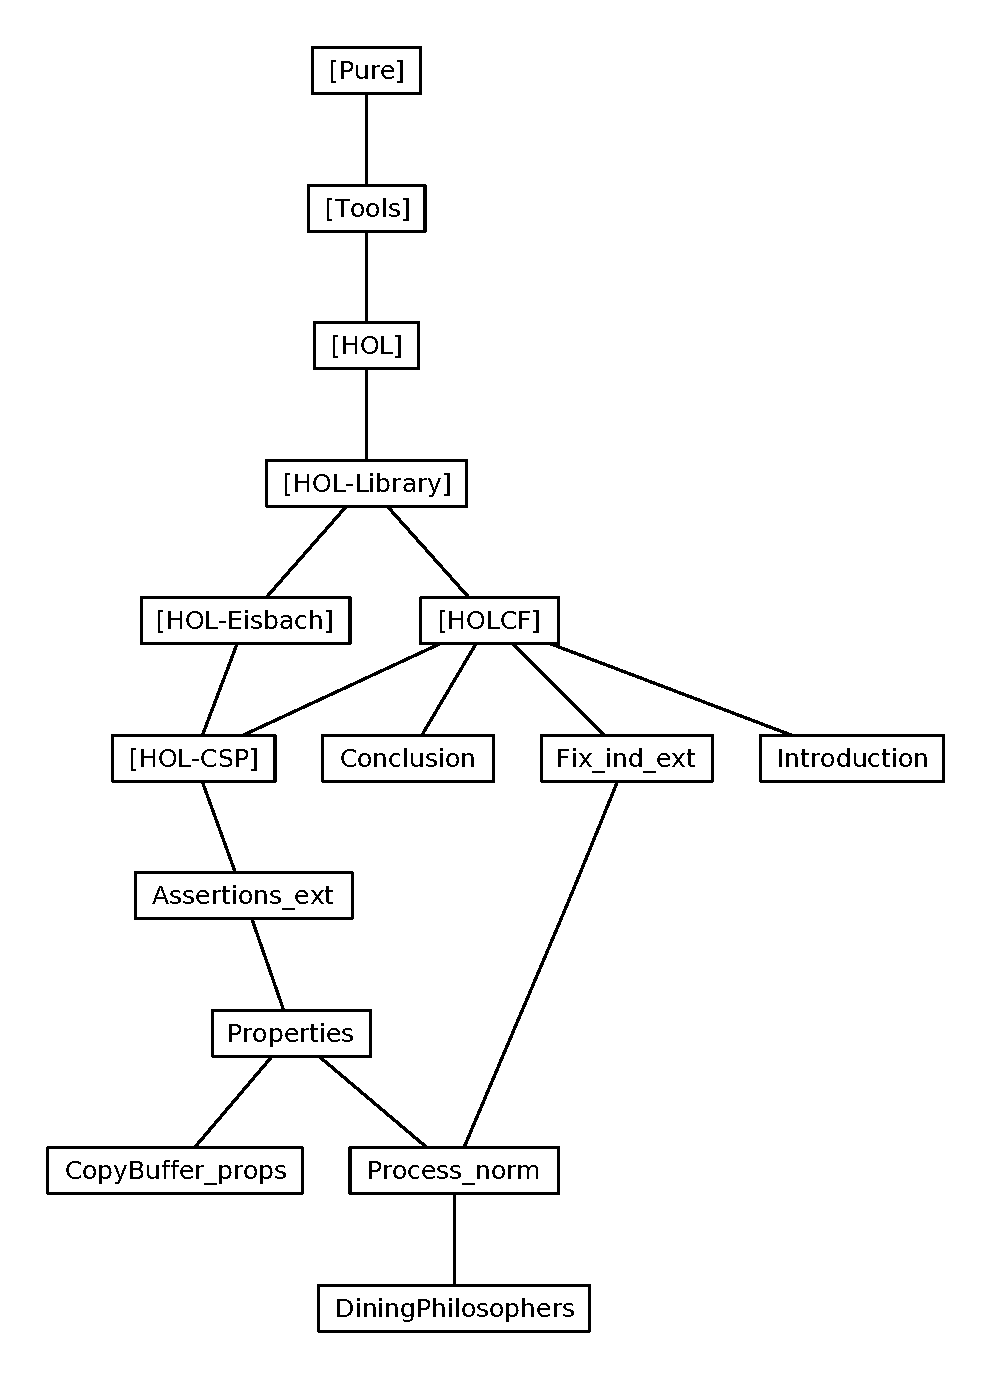
\includegraphics[width=\textwidth]{session_graph}
%\end{center}
%\caption{Theory Dependency Graph\label{theory-deps}}
%\end{figure}

\clearpage
\input{session}

%\newpage
%\nocite{*}
\bibliographystyle{abbrv}
%\bibliographystyle{plain}
\bibliography{root}

\end{document}
